\section{Simulazioni e analisi dei risultati} \label{sec:res_analisys}
Le simulazioni sono state eseguite su una macchina Asus Vivobook S15 avente le seguenti caratteristiche: processore Intel Core i7-8565U 4 core 1.8 GHz; 8GB di RAM; SSD Kingstone da 256 GB.

Tutti i risultati degli esperimenti, come i grafici di andamento medio o le animazioni delle singole simulazioni, sono disponibili sul repository GitHub del progetto \href{https://github.com/leonardo-guglielmi/Multiagent-exploration-system.git}{\textsf{https://github.com/leonardo-guglielmi/Multiagent-exploration-system.git}}.

Negli esperimenti che seguono per ciascun tipo di scenario sono state effettuate 30 prove, ognuna con una configurazione delle posizioni iniziali degli agenti e degli utenti assegnata in modo casuale secondo una distribuzione uniforme lungo l'area di interesse.

\pagebreak
\subsection{Esperimento 1: verifica dell'efficacia dell'algoritmo di esplorazione}\label{subsec:exp1}
In questo esperimento si vuole verificare che l'algoritmo di esplorazione apporti effettivamente un miglioramento in termini di RCR totale rispetto al solo algoritmo per la copertura.
Per confermare ciò sono state effettuate delle simulazioni alternando l'esecuzione del metodo di esplorazione e la presenza delle BS, per un totale di 4 scenari diversi per ciascuna simulazione eseguita, utilizzando la tecnica di campionamento \textit{local}.


Nelle Tabelle  \ref{tab:exp1_cov_statistics}, \ref{tab:exp1_expl_statistics}  si mostrano alcuni indici statistici sui valori finali di RCR ed esplorazione raggiunti, mentre in Figura  \ref{fig:confronto_cov_exp1}, \ref{fig:confronto_expl_exp1}  vengono confrontati gli andamenti medi delle due grandezze durante le simulazioni.
Si osserva che, quando in uso, l'algoritmo di esplorazione effettivamente porta ad avere dei valori finali di copertura migliori. Si nota invece che quando esso non viene eseguito, una volta raggiunta una certa configurazione gli agenti smettono di muoversi, in quanto l'algoritmo di controllo non permette loro di abbandonare la copertura di alcuni utenti per la ricerca di altri, limitando quindi il numero massimo di utenti raggiungibili; a fronte di questo, si ipotizza dunque che se si fosse aumentato il numero di iterazioni di ciascuna simulazione, negli scenari con esplorazione si sarebbero potuti raggiungere valori di copertura migliori.
\begin{table}[t]
\begin{tabular}{|c|c|c|c|c|}
\hline
Simulazione & Massimo & Minimo & Media & Dev. standard \\
\hline
Esplorazione con BS & 0.97 & 0.73 & 0.87 & 0.0645 \\
No esplorazione con BS & 0.93 & 0.63 & 0.79 & 0.0756\\
Esplorazione senza BS & 0.87 & 0.63 & 0.75 & 0.0677 \\
No esplorazione senza BS & 0.8 & 0.5 & 0.64 & 0.0848 \\
\hline
\end{tabular}
\caption{\label{tab:exp1_cov_statistics}Primo esperimento, indici dei valori finali di copertura}
\end{table}

Inoltre, per fornire una migliore interpretazione dei dati, si fa presente che nelle simulazioni senza BS, nella maggior parte dei casi, il numero di agenti risulta troppo basso per avere una qualsiasi configurazione tale da permettere la copertura di tutti gli utenti.

\begin{figure}
    \centering
    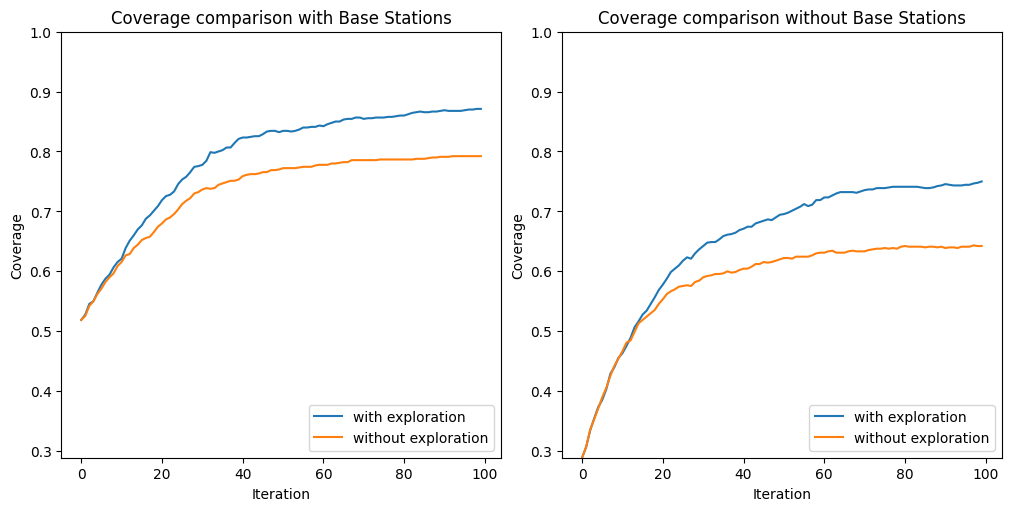
\includegraphics[width=1\textwidth]{img/ch4/experiment1/coverage_comparison.png}
    \caption[Grafici di copertura nel primo esperimento]{Confronto tra gli andamenti medi della copertura negli scenari di simulazione del primo esperimento.}
    \label{fig:confronto_cov_exp1}

    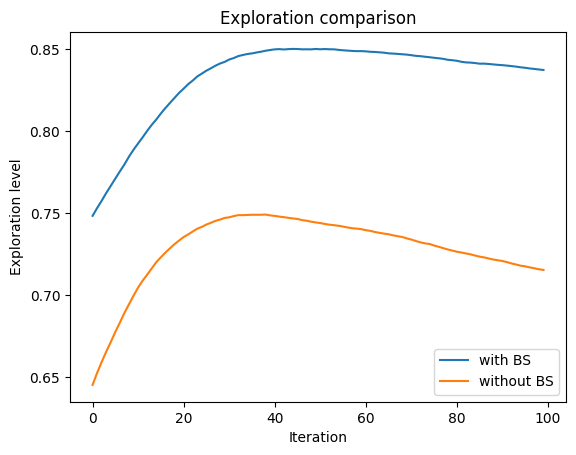
\includegraphics[width=0.5\textwidth]{img/ch4/experiment1/exploration_comparison.png}
    \caption[Grafici di esplorazione nel primo esperimento]{Confronto tra gli andamenti medi dell'esplorazione negli scenari di simulazione del primo esperimento.}
    \label{fig:confronto_expl_exp1}
\end{figure}

\begin{table}[t]
\centering
\begin{tabular}{|c|c|c|c|c|}
\hline
Simulazione & Massimo & Minimo & Media & Dev. standard \\
\hline
Con BS & 0.87 & 0.81 & 0.83 & 0.0129 \\
Senza BS & 0.76 & 0.67 & 0.71 & 0.0198 \\
\hline
\end{tabular}
\caption{\label{tab:exp1_expl_statistics}Primo esperimento, indici dei valori finali di esplorazione.}
\end{table}

\begin{figure}[p]
    \centering
    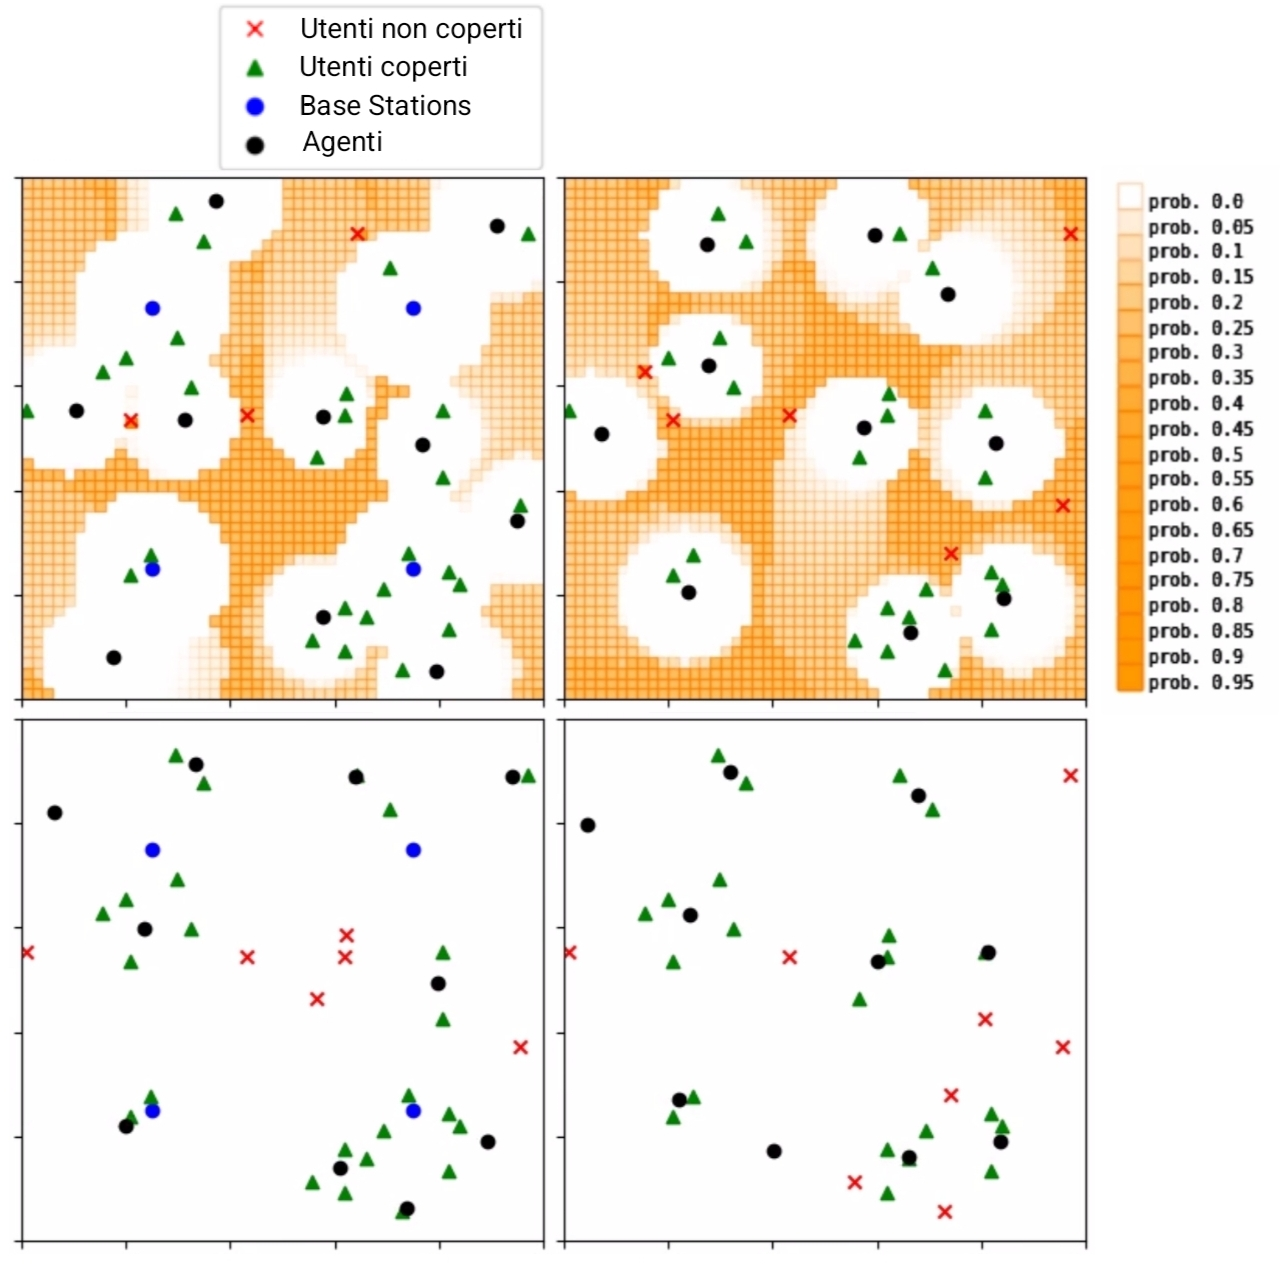
\includegraphics[width=1\linewidth]{img/ch4/experiment1/esempio_simulazioni.jpg}
    \caption[Simulazioni del primo esperimento]{Simulazioni del primo esperimento. In alto a sinistra, lo scenario con esplorazione e con BS; in alto a destra lo scenario con esplorazione ma senza BS; in basso gli scenari senza esplorazione.}
    \label{fig:esempio_simu_exp1}
\end{figure}


\pagebreak
\subsection{Esperimento 2: valutazione del metodo di campionamento migliore}\label{subsec:exp2}
Una volta verificata l'efficacia dell'algoritmo di esplorazione si vuole capire quale, tra le varie tecniche di campionamento, permette di avere dei valori di RCR ed esplorazione migliori.
Data l'uniformità dei risultati precedenti, i seguenti esperimenti sono stati svolti in scenari in cui erano presenti le BS.

\begin{table}[p]
\centering
\begin{tabular}{|c|c|c|c|c|c|}
\hline
Esplorazione & Systematic & Local & Penalty & Ann.forward & Ann.reverse \\
\hline
Massima & 0.86 & 0.87 & 0.86 & 0.87 & 0.86 \\
Minima & 0.79 & 0.79 & 0.79 & 0.81 & 0.81 \\
Media & 0.83 & 0.84 & 0.82 & 0.85 & 0.84 \\
Dev. standard & 0.017 & 0.017 & 0.020 & 0.015 & 0.014 \\
\hline
\end{tabular}
\caption{\label{tab:exp2_expl_statistics}Secondo esperimento, indici dei valori finali di esplorazione.}

\vspace*{0.5 cm}

\begin{tabular}{|c|c|c|c|c|c|}
\hline
Copertura & Systematic & Local & Penalty & Ann.forward & Ann.reverse \\
\hline
Massima & 0.97 & 0.97 & 0.93 & 1 & 0.97 \\
Minima & 0.7 & 0.73 & 0.6 & 0.7 & 0.77 \\
Media & 0.83 & 0.86 & 0.82 & 0.86 & 0.88 \\
Dev. standard & 0.067 & 0.060 & 0.087 & 0.072 & 0.056 \\
\hline
\end{tabular}
\caption{\label{tab:exp2_cov_statistics}Secondo esperimento, indici dei valori finali di copertura.}

\vspace*{0.5 cm}

\begin{tabular}{|c|c|c|c|c|c|}
\hline
 & Systematic & Local & Penalty & Ann.forward & Ann.reverse \\
\hline
tempo medio & 849.3 & 384 & 835.3 & 515 & 495.1 \\
\hline
\end{tabular}
\caption{\label{tab:exp2_time comparison}
Secondo esperimento, tempi medi di esecuzione.}
\end{table}

\begin{figure}[p]
    \centering
    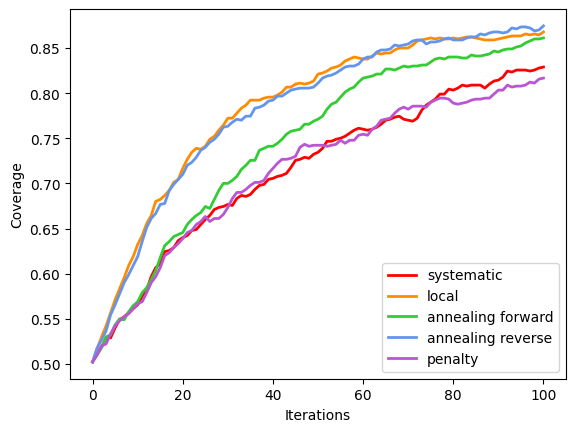
\includegraphics[width=0.8\textwidth]{img/ch4/experiment2/coverages_graphic_comparison.png}
    \caption[Grafici di copertura nel secondo esperimento]{Secondo esperimento, confronto tra i valori medi di copertura utente.}
    \label{fig:confronto_cov_exp2}

\vspace*{0.5cm}

    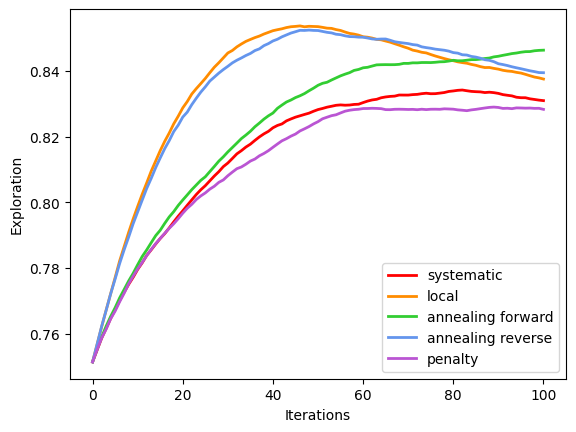
\includegraphics[width=0.8\textwidth]{img/ch4/experiment2/exploration_graphic_comparison.png}
    \caption[Grafici di esplorazione nel secondo esperimento]{Secondo esperimento, confronto dell'andamento medio di esplorazione tra le varie tecniche di campionamento.}
    \label{fig:confronto_expl_exp2}
\end{figure}

Osservando i valori di \textbf{esplorazione} (Figura \ref{fig:confronto_expl_exp2}), si constata che i metodi \textit{local} e \textit{annealing reverse} raggiungo dei livelli molto alti in breve tempo, per poi favorire le posizioni raggiunte dagli agenti.
La tecnica \textit{Annealing forward} invece, a fronte di un transitorio meno rapido, riesce a raggiungere valori finali più alti, come si vede anche in Tabella \ref{tab:exp2_expl_statistics}.
Analizzando i livelli di \textbf{copertura} (Figura \ref{fig:confronto_cov_exp2}), si nota come i metodi \textit{local} e \textit{annealing reverse} risultino i più performanti, sia per i livelli finali raggiunti (Tabella \ref{tab:exp2_cov_statistics}) sia per la velocità di convergenza.
Queste due tecniche sembrano quindi del tutto equivalenti; tuttavia analizzando i tempi di esecuzione in Tabella \ref{tab:exp2_time comparison} si osserva che il tempo della tecnica \textit{local} è circa del 28\% minore rispetto a quello della tecnica \textit{annealing reverse} , portando quindi a favorire la prima per la sua maggiore velocità di esecuzione.

\pagebreak
\subsection{Esperimento 3: variazione della dinamicità dell'ambiente}\label{subsec:exp3}
Fino ad ora gli esperimenti effettuati hanno usato valori di $\mathbb{P_D}$ e $\mathbb{P_B}$ coerenti con un contesto in cui l'informazione relativa al livello di esplorazione in una regione rimane attendibile per un intervallo di tempo relativamente lungo, ovvero coerenti con ambienti aventi bassa dinamicità. 
Con quest'ultimo esperimento dunque si vuole verificare le performance del sistema quando opera in un ambiente maggiormente mutabile nel tempo.
Dati i risultati del precedente esperimento, si è deciso di eseguire queste simulazioni usando solamente la ricerca \textit{local}, confrontando nelle varie prove lo stesso scenario iniziale, ma variando le probabilità di apparizione e disconnessione degli utenti: in un caso si usano i valori definiti in \ref{sec:param_vals}, mentre nell'altro si usano $\mathbb{P_D}=0.01$ e $\mathbb{P_B}=0.07$.

\begin{figure}[p]
    \centering
    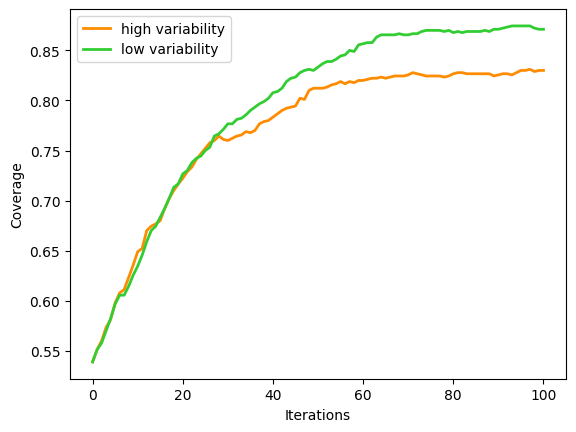
\includegraphics[width=0.8\textwidth]{img/ch4/experiment3/coverages_graphic_comparison.png}
    \caption[Grafici di copertura nel terzo esperimento]{Confronto tra l'andamento medio della copertura negli scenari di simulazione del terzo esperimento.}
    \label{fig:confronto_cov_exp3}

\vspace*{0.5cm}

    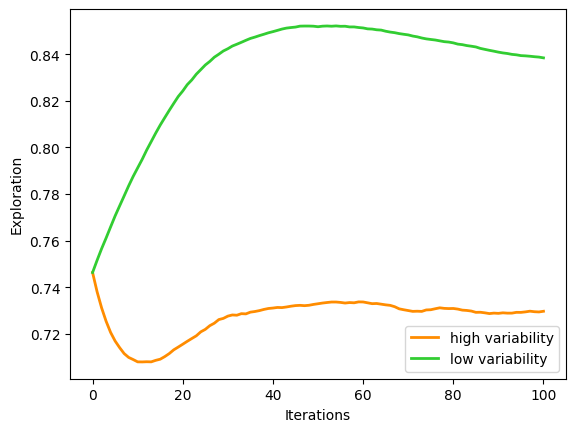
\includegraphics[width=0.8\textwidth]{img/ch4/experiment3/exploration_graphic_comparison.png}
    \caption[Grafici di esplorazione nel terzo esperimento]{Confronto tra l'andamento medio dell'esplorazione negli scenari di simulazione del terzo esperimento.}
    \label{fig:confronto_expl_exp3}
\end{figure}

Analizzando i risultati in Figura \ref{fig:confronto_expl_exp3} notiamo come i livelli di \textbf{esplorazione} diminuiscano drasticamente: questo tuttavia era prevedibile, infatti con questa configurazione la probabilità che appaia un utente in una cella cresce molto rapidamente, e rende impossibile raggiungere alti livelli di esplorazione con la quantità di agenti usati nelle simulazioni.
Per quanto riguarda la \textbf{copertura} (Figura \ref{fig:confronto_cov_exp3}) invece, si riescono a raggiungere dei livelli abbastanza buoni: benché l'algoritmo di esplorazione non impedisca di esplorare ripetutamente alcune zone, è abbastanza flessibile da guidare gli agenti attraverso l'area, disincentivando spostamenti brevi e ripetuti in favore di una traiettoria più pulita.

\begin{figure}
    \centering
    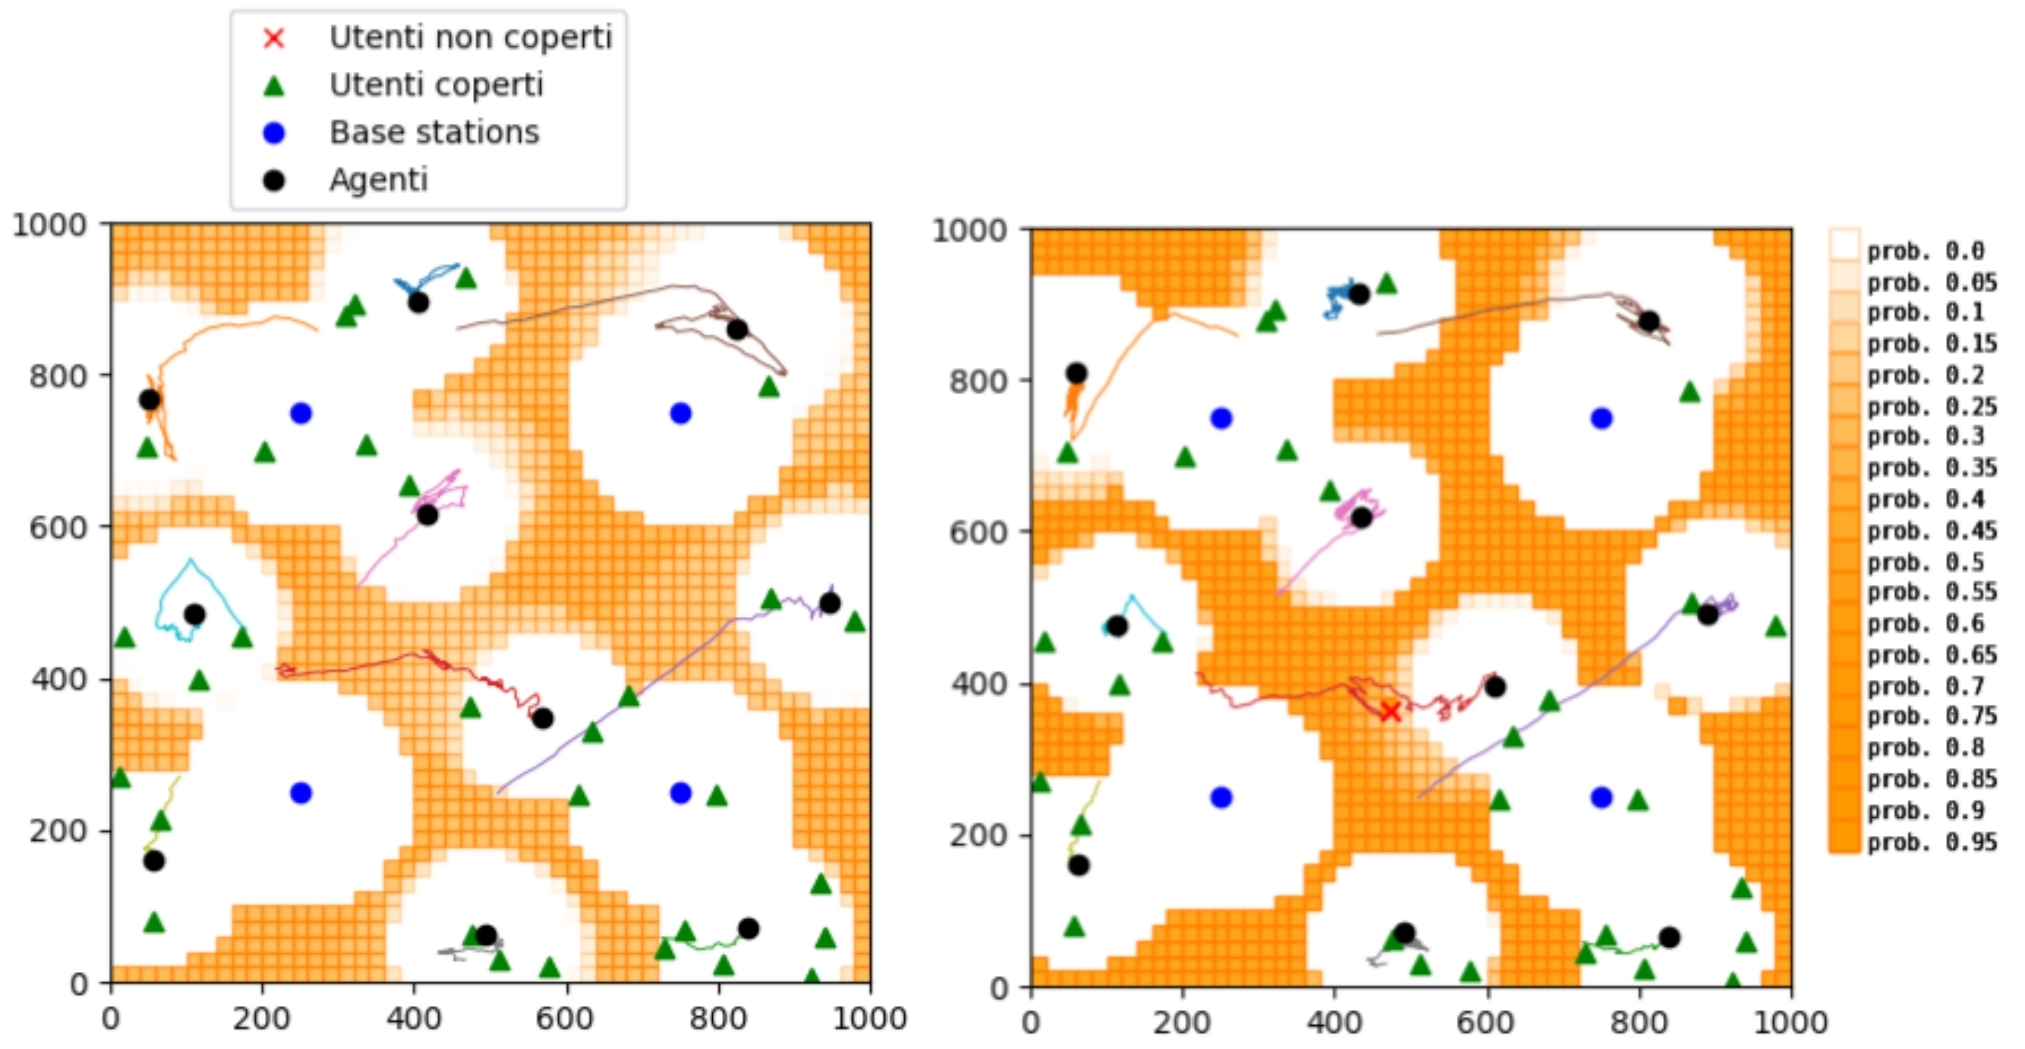
\includegraphics[width=1\linewidth]{img/ch4/experiment3/esempio_exp3_1.jpg}
    \label{fig:esempio_exp3_1}

    \vspace*{0.5cm}
    
    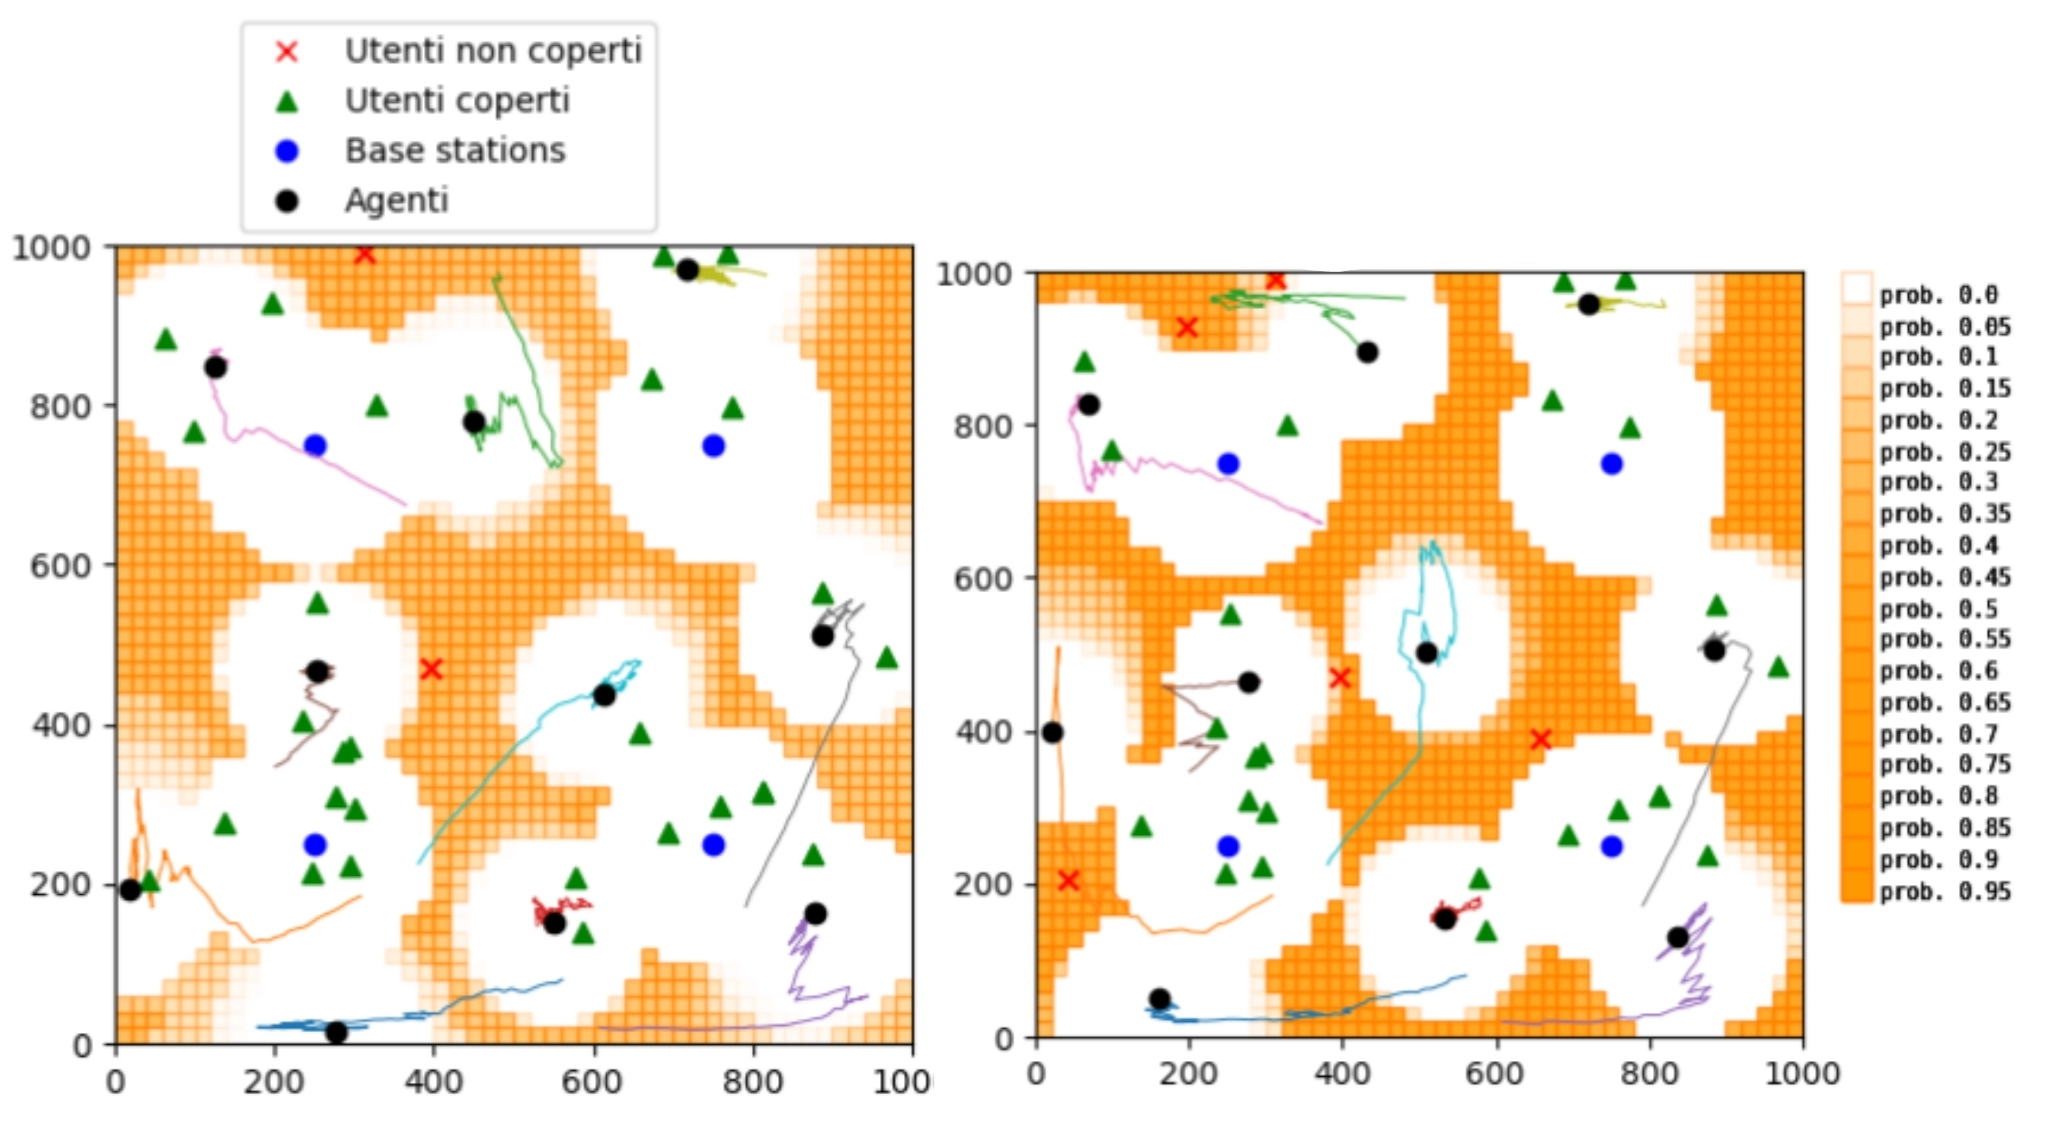
\includegraphics[width=1\linewidth]{img/ch4/experiment3/esempio_exp3_2.jpg}
    \label{fig:esempio_exp3_2}
    \caption[Confronti tra simulazioni con probabilità diverse]{Confronti tra simulazioni con probabilità diverse. Nello scenario di simulazione in alto, nonostante il cambio di parametri le due prove hanno raggiunto livelli di copertura simili. Nello scenario in basso invece la maggiore variabilità dell'ambiente provoca una diminuzione dei risultati raggiunti.}
    
    
\end{figure}
